At the end of this worksheet you should be able to  
\begin{itemize}
	\item calculate stress and strain and use Young's Modulus to solve for an unknown.
	\item plot all relevant quantities of simple harmonic motion over time.
	\item use the quantities of simple harmonic motion and the mathematical description to solve for an unknown.
\end{itemize}


\begin{enumerate}
\setlength\itemsep{2 in}

\item
Consider a wire that is \SI{0.1}{mm} in diameter and \SI{2}{m} long and a Young's Modulus of \SI{120}{\giga \pascal} ($\SI{1}{\giga\pascal}=\SI{e9}{\pascal}$). If you applied \SI{100}{N} to this wire, then what is the stress on the wire? What is the strain? By how much does its length change? What is its new length? What percent change is this?

\item
If instead a \SI{200}{N} force or a \SI{1000}{N} force is applied then what is stress, strain, length change and percent change in the length from its original length?\\

\item
If instead the wire was \SI{1}{m} long with \SI{100}{N} applied, then how much does it stretch? What percent change is this?

\item
What if the wire had half of its cross sectional diameter with \SI{100}{N} applied?

\item 
Now comparing the form of Hooke's Law for springs $F=kx$ to Hooke's Law for stress and strain $\tfrac{F}{A}= Y\tfrac{\Delta l}{L}$, how could you write an expression for spring constant in terms of Young's modulus, length, and cross sectional area? What does this tell you about what would happen to the spring constant of a spring if you cut the spring in half?

\item
Speaking of springs, if you attach two springs to an object side by side, then we say the springs are attached \emph{in parallel}. This will result in two spring forces on the object that has been displaced some distance $x_1$. If you were to model this arrangement of springs in parallel as a single spring with a single spring constant that would have the same effect, then what would this single effective spring constant $k_e$ be in terms of of the original two spring constants $k_1$ and $k_2$? \bigskip

\item
If instead of a \emph{parallel} arrangement, we attach one spring to another spring and then to the object, we say that these springs are connected \emph{in series}. Let's find an expressions for an effective spring constant for this arrangement. Each spring will stretch a different amount based on its spring constant, but the object will experience one force and \emph{both of the springs is exerting the same force.} \bigskip

\item
A wire of length $l_1$ and volume $V$ and cross sectional area $A_1$ is stretched out to length $l_2$, what is its new cross sectional area? Think about this in terms of proportionality.

\item
A \SI{60}{kg} person upright. By how much does the femur shorten if each femur carries half the weight of the person? The cross sectional area of a femur is about \SI{4}{cm^2} and the length is about \SI{30}{cm} Also find the percent change in length. 

\item
A \SI{1}{kg} mass attached to a spring of spring constant $\SI{1000}{N/m}$ is positioned so that the spring is stretched \SI{10}{cm} from its relaxed length. After you finish the following questions, make sure you can write down expressions for all of them in general as well as working them inside out.
\begin{itemize}
	\setlength\itemsep{1 in}
	\item How much spring potential energy does it have at this position?
	\item When it is released, and it heads back toward equilibrium gaining kinetic energy as it does, then what is the maximum kinetic energy it can achieve? How stretched out is the spring when it has this much kinetic energy? 
	\item What is the mass's velocity when it has maximum kinetic energy?
	\item What is the period of this mass's motion? What is its frequency? What is its angular frequency?
	\item What is the force on the mass when it is at its maximum displacement?
	\item What is the force on the mass when it is at the equilibrium position?
	\item What is the maximum acceleration of the mass? Where does this occur?
	\item Where is the mass when its potential energy and kinetic energy at that position are equal?
\end{itemize}

\item
A \SI{1}{kg} mass on a spring has the displacement graph that follows. What is the angular frequency, natural frequency, period, spring constant, amplitude, maximum velocity, maximum acceleration, maximum kinetic energy, maximum potential energy, and total energy? Also fill out the rest of the graphs.\\
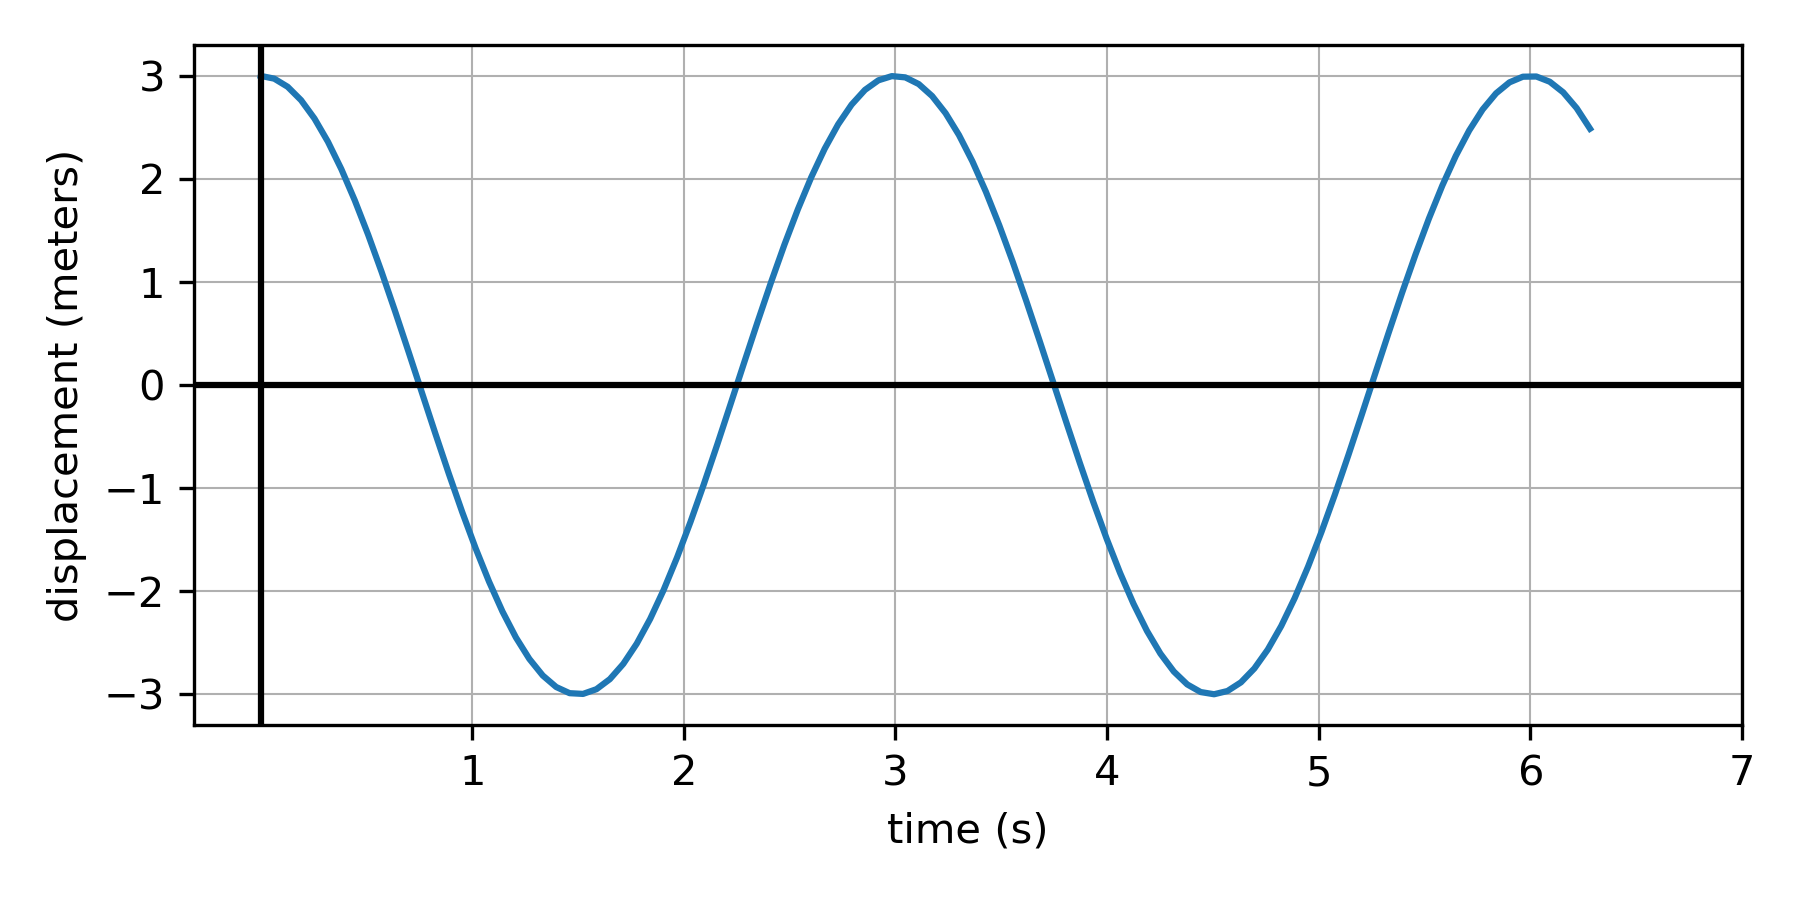
\includegraphics[scale=1]{week11-dispvst.png}\\
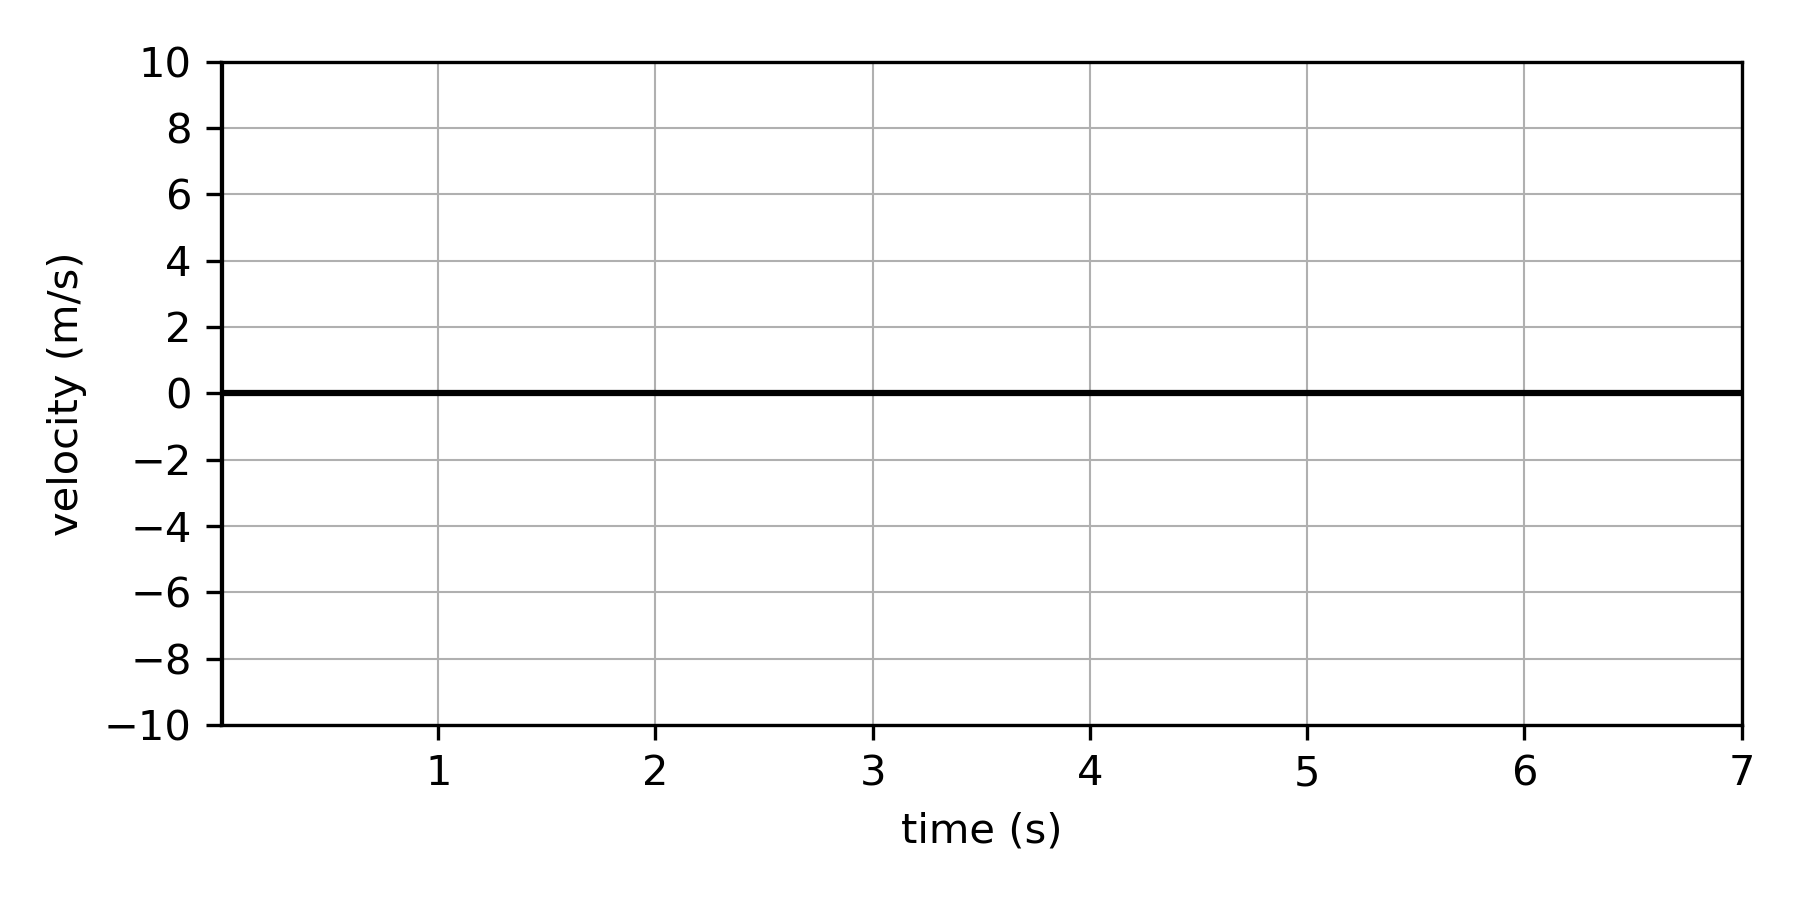
\includegraphics[scale=1]{week11-velvst.png}\\
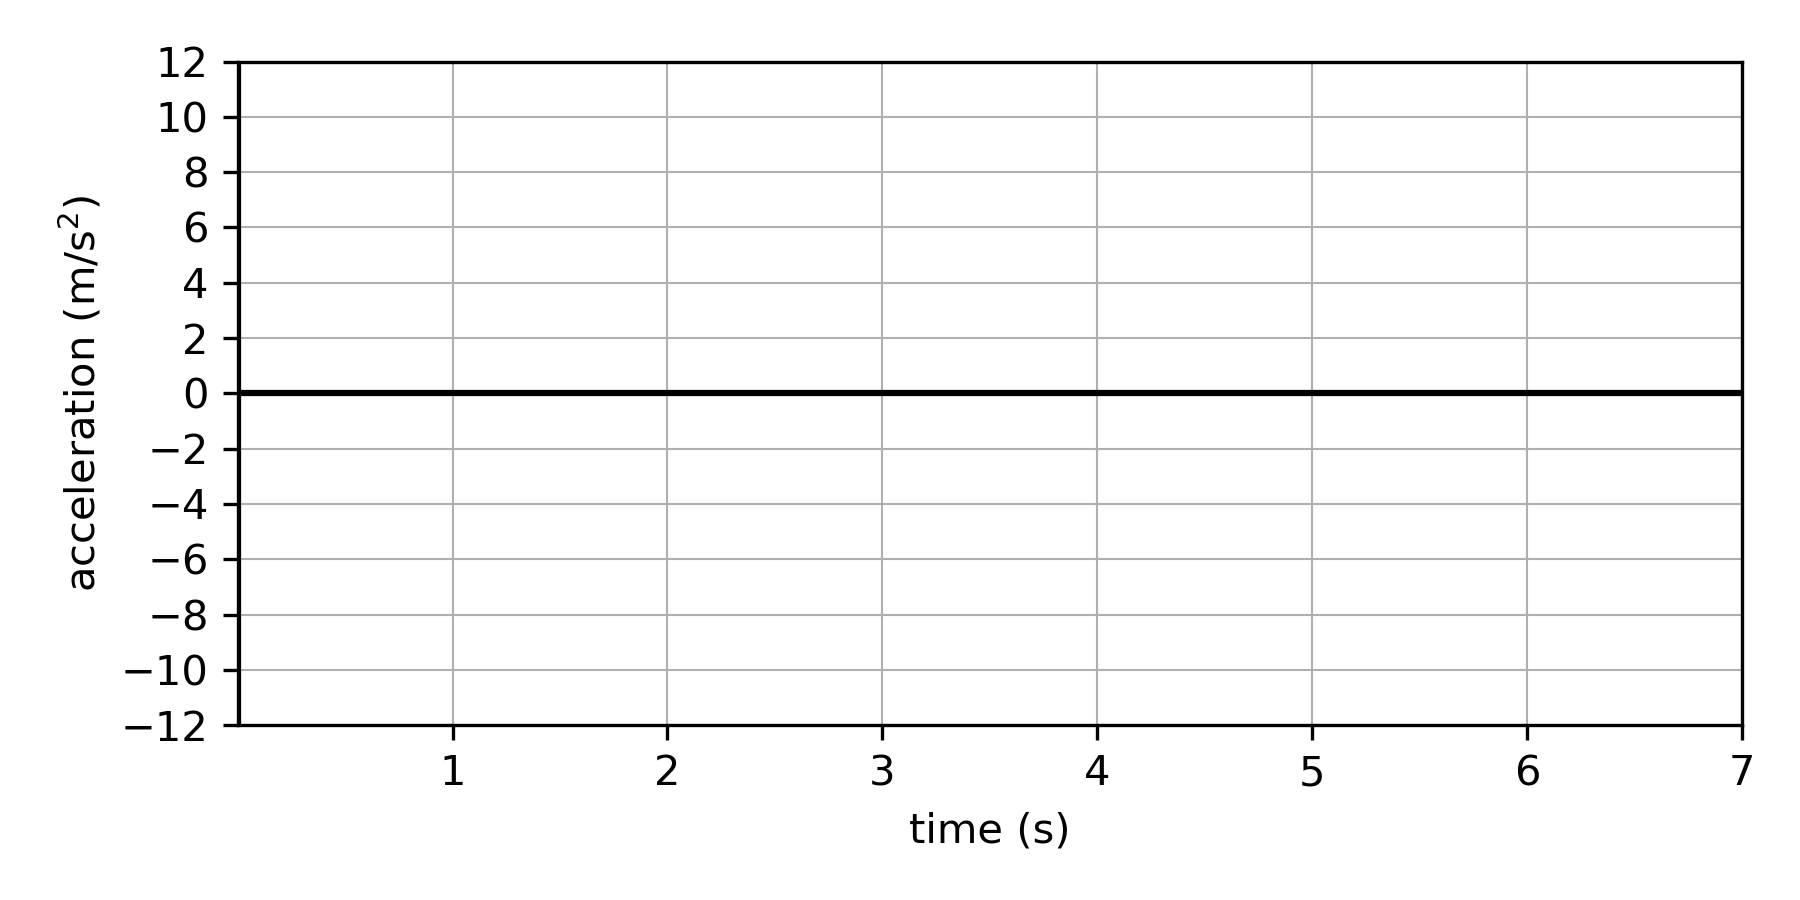
\includegraphics[scale=1]{week11-accvst.png}\\
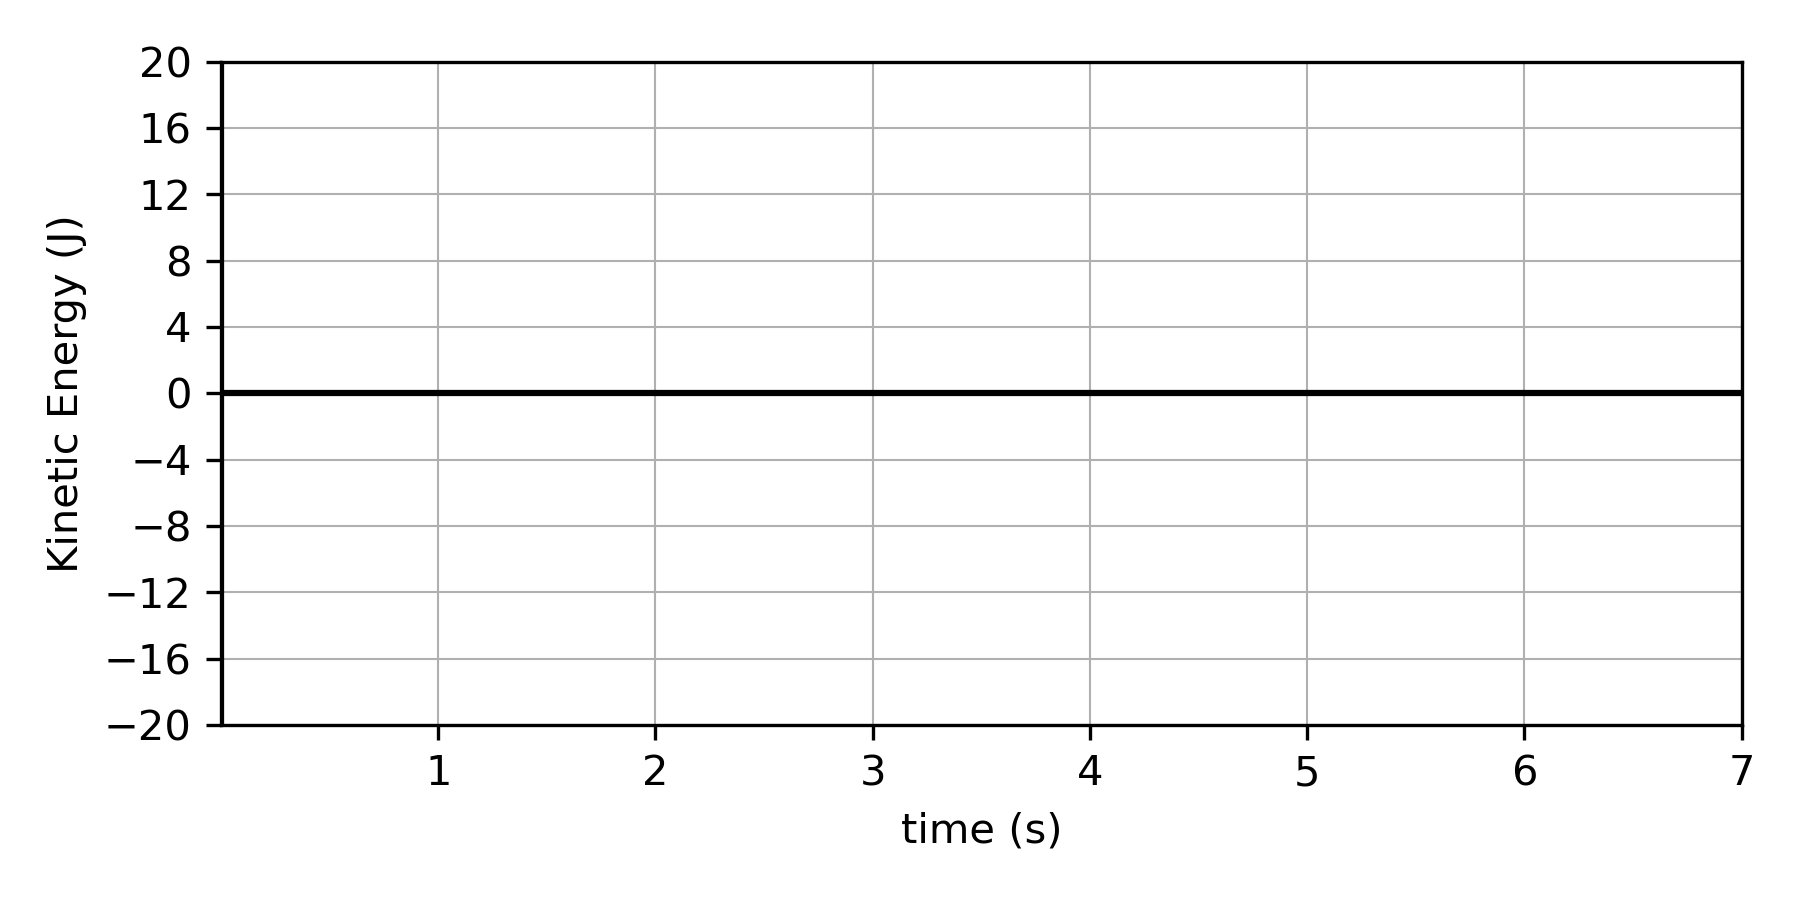
\includegraphics[scale=1]{week11-kevst.png}\\
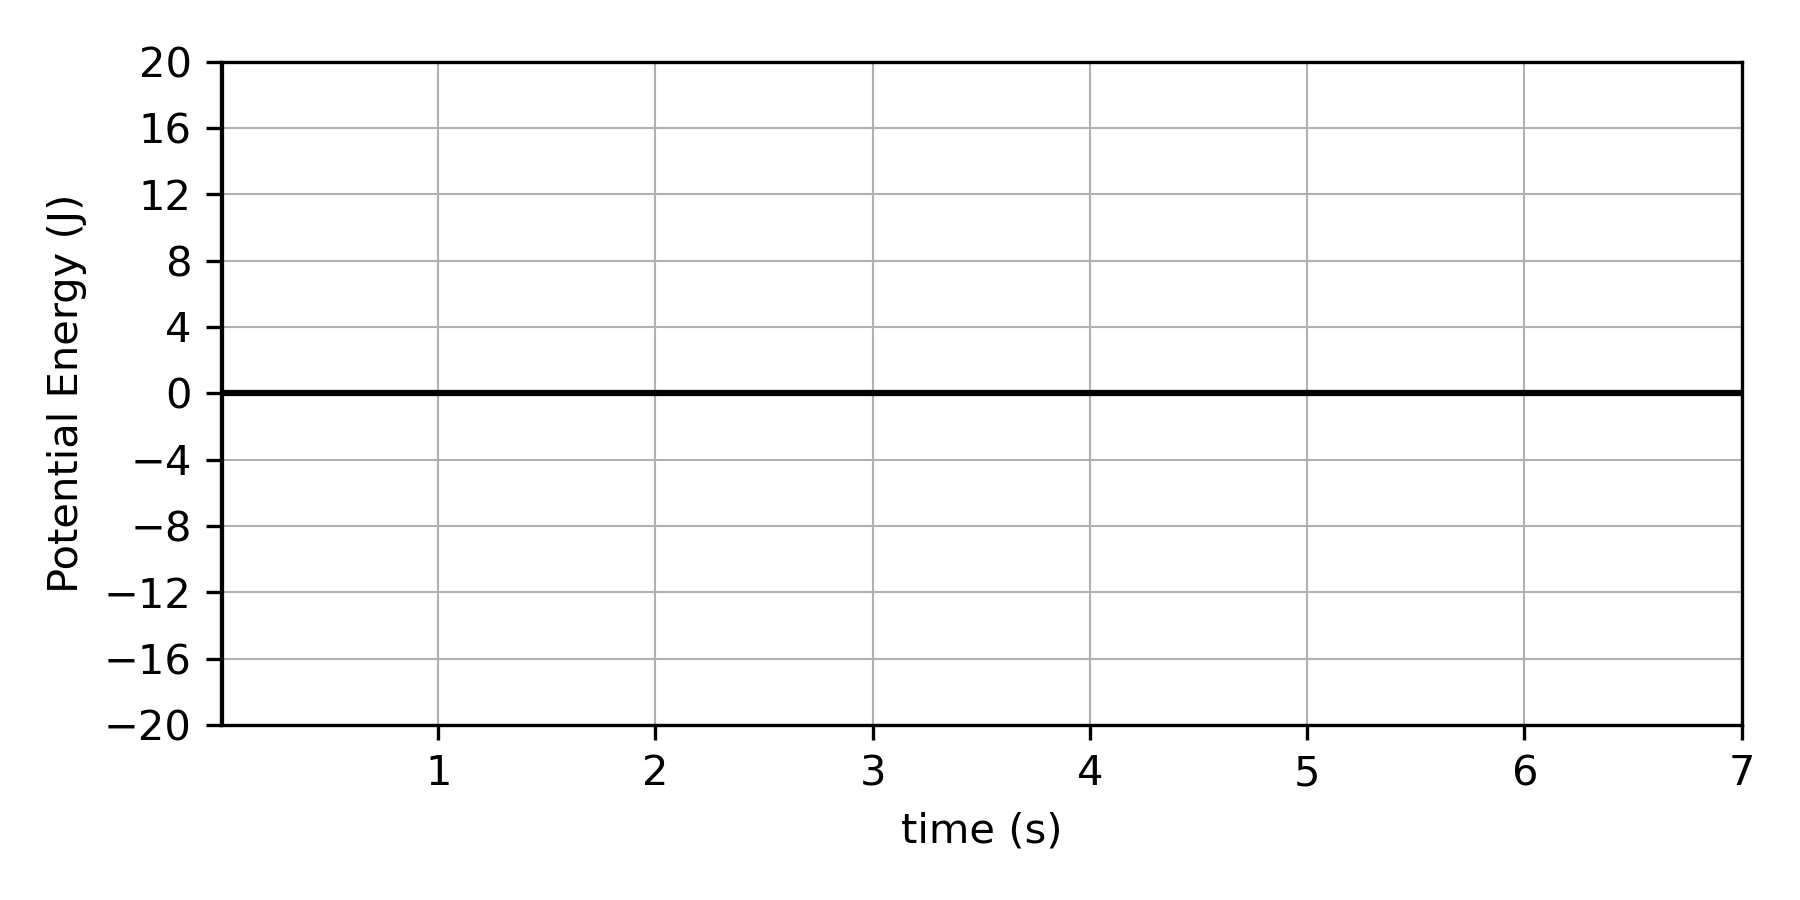
\includegraphics[scale=1]{week11-pevst.png}\\
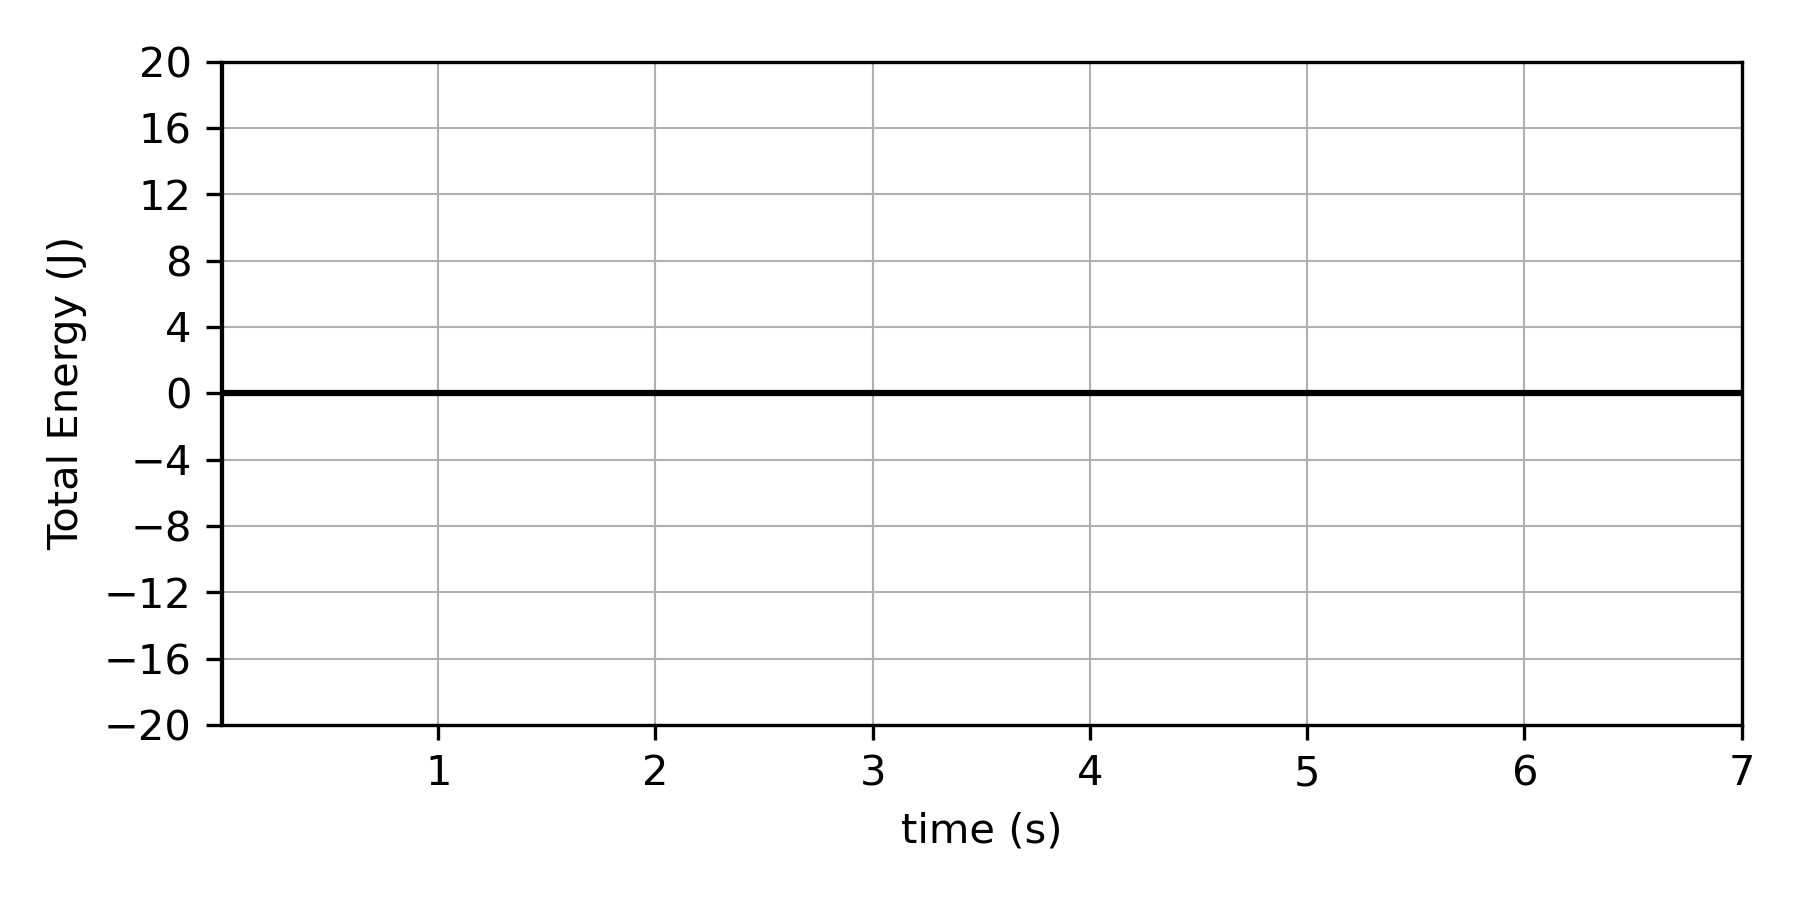
\includegraphics[scale=1]{week11-evst.png}\\


\item
According to the table below, which material stretches more, \SI{2}{m} of steel or \SI{1}{m} of copper of the same width?\bigskip

\item
Four brass wires are subjected to the same tensile stress. The wires have the following unstretched lengths and widths. Rank them in order from least to most change in length.
\begin{enumerate}
	\item length $L$, diameter $d$
	\item length $2L$, diameter $d$
	\item length $4L$, diameter $d/2$
	\item length $L/4$, diameter $d/2$
\end{enumerate}

\item
A \SI{0.5}{\meter} long guitar string of cross sectional area of \SI{1.0e-6}{\meter} and Young's modulus $Y=\SI{2.0}{\giga\pascal}$. By how much must you stretch the string to obtain a tension of \SI{20}{\newton}.

\item
Young's modulus is like the spring constant for materials, but if you stretch a material beyond a limit then the material will not exactly return to its original length. This point of stress is called the \emph{elastic limit} of a material. After this point, \emph{plastic deformation} begins to occur which means the material will be permanently deformed. More stress can be applied beyond this but the material will fracture and break when the stress reaches the \emph{breaking point}. A hair breaks under a tension of \SI{1.2}{\newton} and the tensile stress of the breaking point is \SI{200}{\mega\pascal}. What is the diameter of the hair? \bigskip

\item
A copper wire of length \SI{3.0}{\meter} is observed to stretch by \SI{2.1}{\milli\meter} when a weight of \SI{120}{\newton} is hung from the end. What is the diameter of the wire and what is the stress in the wire? If the breaking point of copper is \SI{400}{\mega\pascal}, what is the maximum weight that may be hung from this wire?





\newpage 

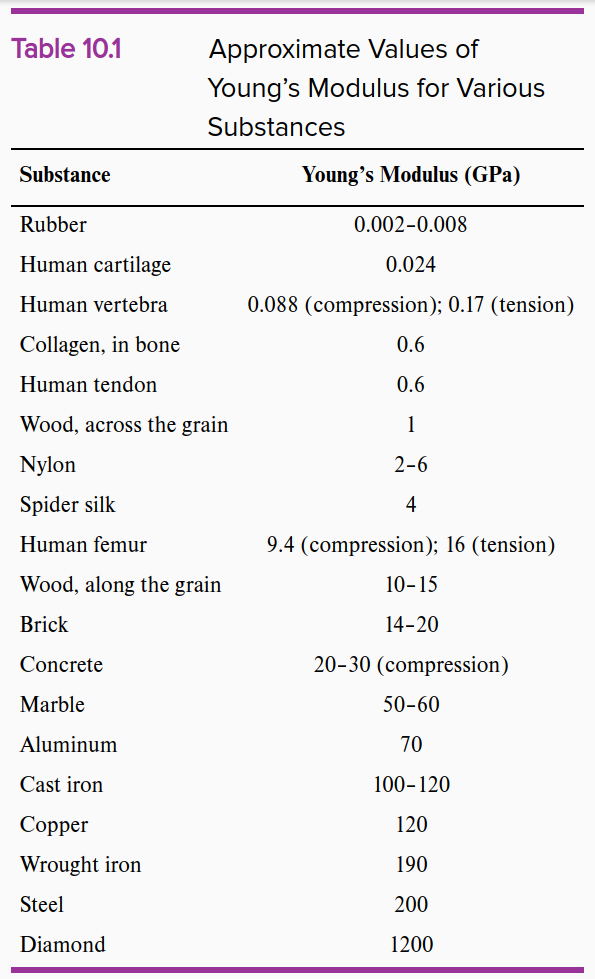
\includegraphics[scale=0.35]{week12-youngs-moduli.png}



\end{enumerate}